%%%%%%%%%%%%%%%%%%%%%%%%%%%%%%%%%%%%%%%%%%%%%%%%%%%%%%%%%%%%%%%%%%%
%                                                                 %
%  GEANT manual in LaTeX form                                     %
%                                                                 %
%  Michel Goossens (for translation into LaTeX)                   %
%  Version 1.00                                                   %
%  Last Mod. Jan 24 1991  1300   MG + IB                          %
%                                                                 %
%%%%%%%%%%%%%%%%%%%%%%%%%%%%%%%%%%%%%%%%%%%%%%%%%%%%%%%%%%%%%%%%%%%
\Documentation {M.Maire}       
\Submitted{01.10.84}                \Revised{20.03.94}
\Version{Geant 3.11}\Routid{BASE020}
\Makehead{The data structures and their relationship}
\section{Dynamic memory}
 
The {\tt GEANT} data structures are stored in the
common \FCind{/GCBANK/} accessible through the following Patchy sequence:
The \FCind{/GCLINK/} variables are pointers to the {\tt GEANT} data structures 
in the \FCind{/GCBANK/} common. 
They belong to a permanent area declared in 
\Rind{GZINIT}.
\FComm{GCBANK}{Dynamic core for the GEANT data structures}
\begin{verbatim}
      PARAMETER (KWBANK=69000,KWWORK=5200)
      COMMON/GCBANK/NZEBRA,GVERSN,ZVERSN,IXSTOR,IXDIV,IXCONS,FENDQ(16)
     +             ,LMAIN,LR1,WS(KWBANK)
      DIMENSION IQ(2),Q(2),LQ(8000),IWS(2)
      EQUIVALENCE (Q(1),IQ(1),LQ(9)),(LQ(1),LMAIN),(IWS(1),WS(1))
      EQUIVALENCE (JCG,JGSTAT)
      COMMON/GCLINK/JDIGI ,JDRAW ,JHEAD ,JHITS ,JKINE ,JMATE ,JPART
     +      ,JROTM ,JRUNG ,JSET  ,JSTAK ,JGSTAT,JTMED ,JTRACK,JVERTX
     +      ,JVOLUM,JXYZ  ,JGPAR ,JGPAR2,JSKLT
C
\end{verbatim}
The figure on the next page indicates the ralations between the  
{\tt GEANT} data structures. 
Detailed description of the data structure parts can be found
in the following sections:
\begin{center}\tt\begin{tabular}{lllrrr}
JRUNG    &[BASE299]        \\
JPART   &[CONS399]        &JMATE    &[CONS199]  \\
JROTM   &[GEOM299]        &JTMED    &[CONS299]  \\
JVOLUM  &[GEOM199]        \\
JSET    &[HITS199]        &JDRAW    &[DRAW399]  \\
JHEAD   &[BASE299]        &JKINE    &[KINE199]  &  JVERTX & [KINE199]\\
JSTAK   &[TRAK399]        \\
IDIGI   &[HITS399]        &JHITS    &[HITS299]  &  JXYZ   & [TRAK 499]
\end{tabular}
\end{center}
\begin{figure}[hbt]
     \centering
     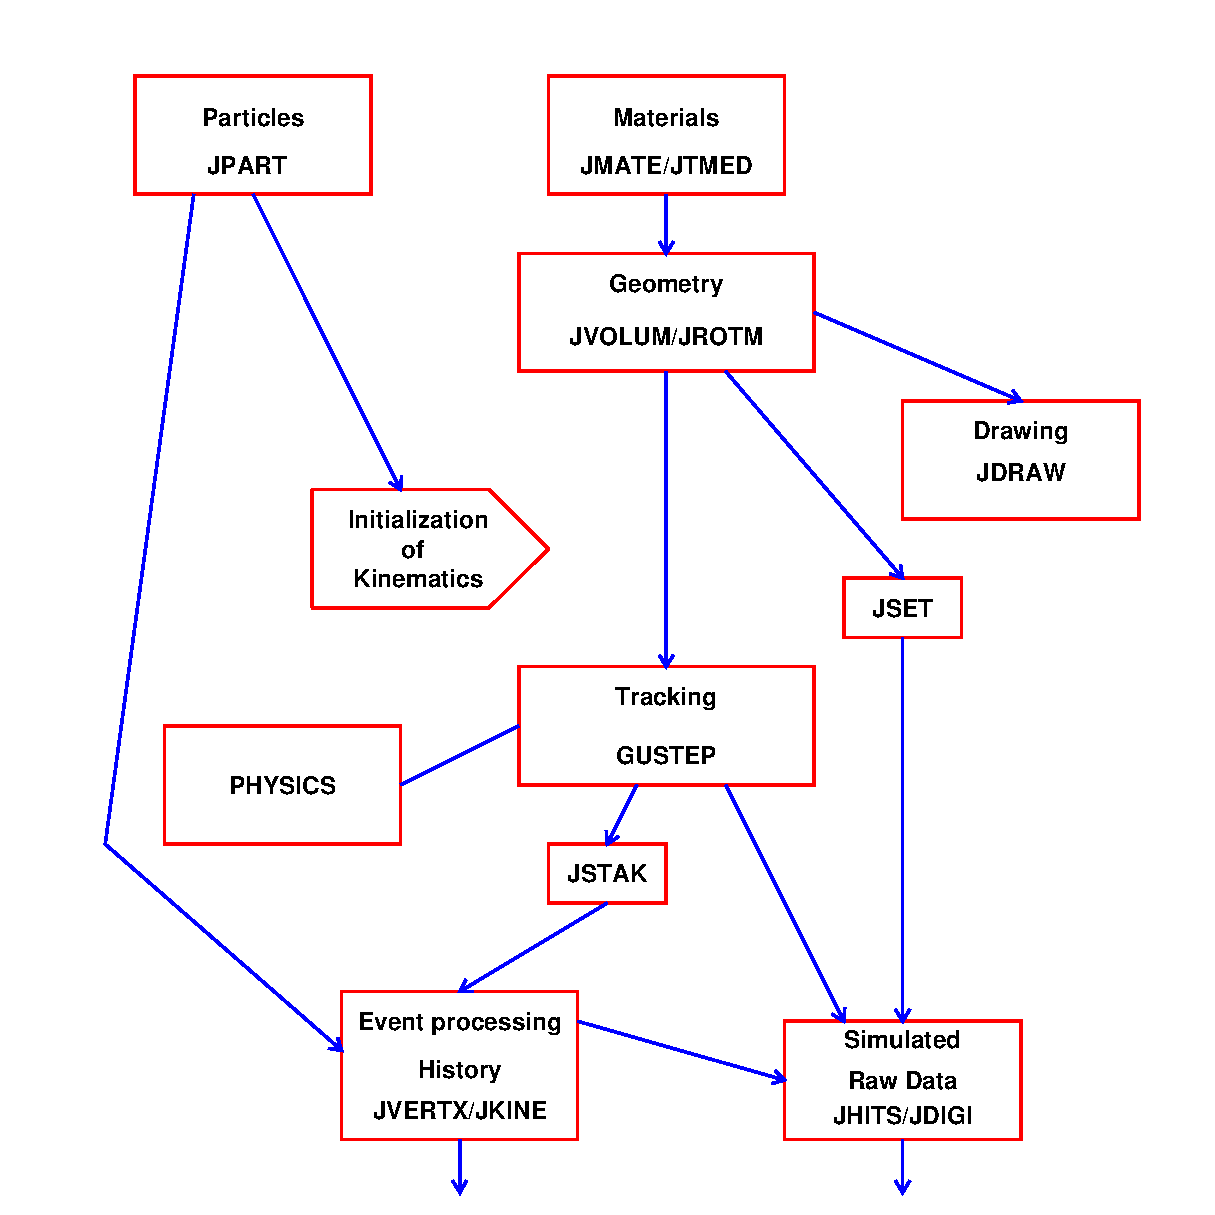
\epsfig{file=eps/base020-1.eps,width=12cm}
     \caption{Relation between {\tt GEANT} data structures}
     \label{fg:base020-1}
\end{figure}
\newpage

\section{Common blocks}
The communication between program segments of the {\tt GEANT} system
is assured by the contents of the data structures and by the definition
of {\it long range} variables in several common blocks.
In addition, within the program segments,
the subroutines communicate with each other through actual arguments
and through the common block variables. A detailed list of the 
user accessed common blocks is given in  {\tt [ZZZZ010]}. 
Their also the variables initialized in \Rind{GINIT} and the possibility
in overriding them through data records {\tt [BASE040]} or 
interactive commands {\tt [XINT]} are specified.
 
In most of the cases there is a correspondence between a
given data structure and a given common block where the current contents of
the banks are stored.
The labelled common blocks are accessible through Patchy/CMZ sequences
identified by the name of the {\tt COMMON}. They are defined in the Patch
\Rind {GCDES}.
 
{\bf Note:}
 
Unless otherwise specified, the long range variables are
initialised in \Rind{GINIT}. When non-zero, default values are
quoted between brackets. If the value may be modified
the keyword for the data record and for the interactive
command is also given in bold characters between brackets.
 

 
 
